% !TeX root = _main.tex
% FILE DIEU PHOI 2/2: thu tu ghep, tai lieu tham khao, phu luc chung.
% Nguoi ghep bai quan ly file nay. KHONG viet lai noi dung cua cac role o day.
% Role 1: muc 1--4; Role 2: muc 5--6; Role 3: muc 7--9.
% !TeX root = _main.tex
% ROLE 1 -- BOI CANH, HE THONG DICH VU, QUY TRINH AS-IS (muc 1--4).
% Nguoi nhan: nhom tu dien. Muc tieu: 4--6 trang noi dung chinh.
% DUOC SUA: file nay, figures/r1_*; nhan \label bat dau bang r1:.
% KHONG SUA: role_2.tex, role_3.tex, _main.tex, _content.tex, analysis/.
% DAU VAO: rubric, PDF Checkpoint 2, CheckPoint1/sections, figures/framework_cp1.png.
% BAN GIAO: pham vi tram do Wq, Resource Map, BPMN AS-IS, nguyen nhan -> bien do.
% HOAN THANH KHI: co BPMN dung ky phap, nguon/nhan AI, khong con TODO role 1.

\section{Bài toán và phạm vi nghiên cứu}
\label{r1:scope}
\subsection{Vấn đề dịch vụ và câu hỏi phân tích}
Dự án xét dịch vụ tiếp nhận triệu chứng trực tuyến, hỗ trợ tổng hợp thông tin,
nhân viên y tế xem xét và hướng dẫn đặt lịch khám khi phù hợp. Báo cáo
Checkpoint 2 đã mô tả hành trình từ khai báo đến xác nhận lịch và chỉ ra điểm
chờ khi hồ sơ được chuyển cho nhân viên y tế~\cite{checkpoint2}.
Báo cáo cuối kỳ tập trung vào một bài toán: thời gian chờ tại trạm tiếp nhận,
phân loại yêu cầu tư vấn và cách phân bổ nhân lực theo khung giờ.

\textbf{Câu hỏi phân tích.} Trong cùng một cấu hình nhu cầu giả định, thay đổi
số điều dưỡng theo giờ và giảm thời gian xử lý hồ sơ có thể giảm thời gian
chờ đến mức nào, với chi phí nhân lực và rủi ro vận hành nào?
Giá trị kỳ vọng là phản hồi kịp thời hơn cho người dùng và sử dụng nguồn lực
phù hợp với thời điểm phát sinh nhu cầu. Kết quả được đánh giá bằng mô phỏng;
chưa phải kết quả triển khai tại cơ sở y tế.

\subsection{Ranh giới hệ thống và ranh giới phép đo}
\begin{table}[htbp]\centering\small
\caption{Phạm vi dịch vụ và phạm vi mô hình định lượng}\label{r1:boundary}
\begin{tabularx}{\linewidth}{@{}p{32mm}Y@{}}
\toprule
Thành phần & Mô tả \\
\midrule
Người sử dụng & Người bệnh hoặc người nhà được ủy quyền khai báo triệu chứng. \\
Tác nhân cung cấp & Điều dưỡng, bác sĩ, nhân viên tiếp nhận và đơn vị vận hành nền tảng. \\
Trigger dịch vụ & Hệ thống nhận mô tả triệu chứng qua ứng dụng. \\
Outcome dịch vụ & Hướng dẫn đã được nhân viên y tế duyệt; xác nhận lịch nếu cần khám và có chỗ. \\
Đầu vào mô hình & Hồ sơ sẵn sàng vào hàng đợi tại trạm điều dưỡng. \\
Đầu ra mô hình & Điều dưỡng hoàn tất xử lý tại trạm; chưa bao gồm toàn bộ thời gian tới khi có lịch khám. \\
Ngoài mô hình & Chẩn đoán, điều trị, thanh toán, công suất bác sĩ và lịch khám phía sau; chất lượng phân loại của AI. \\
\bottomrule
\end{tabularx}
\end{table}
Ứng dụng có thể tiếp nhận thông tin ngoài giờ, nhưng mô phỏng hiện tại chỉ
sinh yêu cầu trong khoảng 07:00--19:00. Việc quy đổi yêu cầu ngoài giờ thành
hàng đợi đầu ngày chưa được mô hình hóa. Nhóm ưu tiên P1 là nhãn của mô hình;
không đồng nhất nó với quy trình xử lý cấp cứu trong toàn bộ dịch vụ.
\todo{1}{Chốt điểm bắt đầu/kết thúc của tác vụ điều dưỡng trên BPMN để khớp với
\texttt{t\_arrival}, \texttt{t\_start}, \texttt{t\_end} ở role 2.}

\section{Mô hình hệ thống dịch vụ}
\label{r1:system}
Báo cáo dùng mô hình hệ thống dịch vụ làm khung chủ đạo để liên kết tác nhân,
nguồn lực, hoạt động, thông tin, quy tắc và kết quả. Góc nhìn đồng tạo giá trị
được dùng để giải thích quan hệ giữa các bên trong cùng khung, theo yêu cầu
một khung phân tích chính của rubric~\cite{rubric}.
\begin{table}[htbp]\centering\small
\caption{Các thành phần của hệ thống và liên hệ với bài toán chờ}
\begin{tabularx}{\linewidth}{@{}p{30mm}Y Y@{}}
\toprule
Thành phần & Biểu hiện trong dịch vụ & Liên hệ với phân tích \\
\midrule
Con người & Người khai báo, điều dưỡng, bác sĩ, tiếp nhận & Số kênh điều dưỡng hoạt động $c_t$. \\
Hoạt động & Thu thập, kiểm tra, phân loại, chuyển tiếp & Thời gian xử lý $S$ và điểm bàn giao. \\
Thông tin & Triệu chứng, tiền sử, mức ưu tiên, trạng thái & Tính đầy đủ có thể làm thay đổi $S$; chưa đo tỷ lệ lỗi. \\
Công nghệ & Biểu mẫu, công cụ tổng hợp, hàng đợi, thông báo & Hỗ trợ nhân viên tiếp nhận thông tin; không suy ra độ chính xác lâm sàng. \\
Quy tắc & Thứ tự xử lý, phân quyền, ngưỡng cảnh báo & FCFS hoặc ưu tiên không chen ngang; mục tiêu thời gian chờ. \\
Kết quả & Hồ sơ được xử lý và chuyển đúng bước & $W_q$, P90, tỷ lệ vượt ngưỡng và chi phí quy ước. \\
\bottomrule
\end{tabularx}
\end{table}
\todo{1}{Bổ sung nguồn học thuật đã đọc cho khung được chọn; dùng thuật ngữ nhất
quán với bài giảng và sơ đồ. Gửi khóa trích dẫn cho người ghép bài.}

\section{Bản đồ nguồn lực và cơ chế đồng tạo giá trị}
\label{r1:resources}
\begin{figure}[htbp]\centering
\includegraphics[width=0.94\linewidth,height=0.48\textheight,keepaspectratio]{figures/framework_cp1.png}
\caption{Bản đồ nguồn lực kế thừa từ Checkpoint 1, cần rà soát theo phạm vi cuối kỳ.}
\label{r1:resource-map}
\source{hình \texttt{framework\_cp1.png} có sẵn trong dự án; lịch sử hỗ trợ AI cần nhóm xác nhận}
\end{figure}
Người sử dụng cung cấp thông tin và phối hợp trả lời; nhân viên y tế đóng góp
tri thức và thời gian; cơ sở khám cung cấp năng lực tiếp nhận; đơn vị vận hành
cung cấp hạ tầng và cơ chế phối hợp. Giá trị xuất hiện khi các nguồn lực được
kết nối thành một yêu cầu có đủ thông tin để xử lý và chuyển tiếp.

Chậm phản hồi có thể phát sinh khi thời gian điều dưỡng không khớp nhu cầu
theo giờ. Thông tin thiếu làm tăng công việc bổ sung và có thể kéo dài xử lý.
Hai cơ chế này tương ứng với hai biến quyết định trong mô hình: $c_t$ và
$E[S]$. Tuy nhiên, mức giảm $E[S]$ nhờ công cụ hỗ trợ hiện là giả định;
bản đồ nguồn lực tự nó không chứng minh hiệu quả của công cụ.
\todo{1}{Hoàn thiện Resource Map: đánh dấu ranh giới, 3--5 nhóm nguồn lực,
mũi tên trao đổi, chú giải và lợi ích/chi phí/rủi ro. Nếu vẽ lại, lưu
\texttt{figures/r1\_resource\_map.pdf} và thay hình trên.}

\section{Quy trình hiện tại và chẩn đoán điểm nghẽn}
\label{r1:asis}
\subsection{Journey và Service Blueprint AS-IS}
Hành trình tham chiếu gồm khai báo triệu chứng, hỏi bổ sung, chờ duyệt,
nhận hướng dẫn, chọn lịch và xác nhận lịch~\cite{checkpoint2}. Hai điểm cần
theo dõi là thiếu thông tin khi khai báo và không biết tiến độ trong lúc chờ.
Blueprint cần nối các hành động này với xử lý phía sau, thay vì chỉ liệt kê
các màn hình ứng dụng.
\begin{table}[htbp]\centering\small
\caption{Tóm tắt các lớp của blueprint tại điểm chờ}
\begin{tabularx}{\linewidth}{@{}p{36mm}Y@{}}
\toprule
Lớp & Nội dung ở bước chuyển hồ sơ cho điều dưỡng \\
\midrule
Evidence & Mã hồ sơ, trạng thái tiếp nhận và kết quả phản hồi. \\
Customer actions & Gửi hồ sơ, theo dõi, cung cấp thông tin bổ sung. \\
Frontstage & Hiển thị trạng thái; nhân viên tương tác khi cần bổ sung. \\
Backstage & Kiểm tra hồ sơ, xếp hàng, điều dưỡng tiếp nhận và chuyển tiếp. \\
Support processes & Lịch trực, phân quyền, lưu dấu thời gian và thông báo. \\
\bottomrule
\end{tabularx}
\end{table}
\todo{1}{Bổ sung hoặc chuyển Journey/Blueprint từ PDF mẫu; chỉ rõ line of
interaction, line of visibility và ít nhất hai pain points. Không gọi bảng
tóm tắt này là sơ đồ blueprint hoàn chỉnh.}

\subsection{BPMN AS-IS và ngoại lệ}
\IfFileExists{figures/r1_bpmn_asis.pdf}{%
\begin{figure}[htbp]\centering
\includegraphics[width=\linewidth,height=0.65\textheight,keepaspectratio]{figures/r1_bpmn_asis.pdf}
\caption{BPMN AS-IS của quy trình tiếp nhận và phân loại.}\label{r1:bpmn}
\end{figure}
}{\placeholder{BPMN AS-IS -- role 1}{Xuất sơ đồ thành
\texttt{figures/r1\_bpmn\_asis.pdf}; báo cáo sẽ tự chèn khi file tồn tại.
Cần có start/end, lane/pool, task, gateway khi có rẽ nhánh, nhánh thiếu
thông tin và điểm bàn giao vào hàng đợi.}}
\todo{1}{Đối chiếu \texttt{assests/diagram.bpmn} và các sơ đồ checkpoint;
chọn đúng AS-IS. Kiểm tra sequence flow trong pool, message flow giữa pool,
nhánh ngoại lệ và ghi nguồn/AI ngay dưới sơ đồ.}

\subsection{Từ điểm nghẽn đến biến đo}
\begin{table}[htbp]\centering\small
\caption{Các giả thuyết chẩn đoán cần đối chiếu với dữ liệu}
\begin{tabularx}{\linewidth}{@{}Y Y Y@{}}
\toprule
Điểm trên quy trình & Cơ chế giả định & Biến kiểm tra \\
\midrule
Chờ điều dưỡng nhận hồ sơ & Công suất cố định trong khi nhu cầu biến thiên & $\lambda_t$, $c_t$, $\rho_t$, $W_q$. \\
Yêu cầu bổ sung thông tin & Thiếu dữ liệu làm kéo dài thao tác & $E[S]$, CV; mô hình chưa tách riêng vòng rework. \\
Hồ sơ ưu tiên chờ cùng hàng & FCFS không phản ánh mức ưu tiên & $W_q$ theo P1/P2/P3. \\
Chuyển tiếp sang lịch khám & Có thể có điểm nghẽn sau trạm điều dưỡng & Cần dữ liệu riêng; ngoài mô phỏng hiện tại. \\
\bottomrule
\end{tabularx}
\end{table}

\FloatBarrier
\clearpage
% !TeX root = _main.tex
% ROLE 2 -- DU LIEU, MO HINH, KIEM CHUNG, AS-IS, MO HINH MO RONG (muc 5--7).
% Nguoi nhan: nhom tu dien. Muc tieu: 5--7 trang noi dung chinh.
% DUOC SUA: file nay, figures/r2_*; nhan \label bat dau bang r2:.
% analysis/ do role 2 dau moi quan ly; bao role 3 truoc khi sinh lai dau ra.
% DAU VAO: analysis/run_analysis.py, extension_analysis.py, data/run_log.txt, data/ext_run_log.txt.
% BAN GIAO: tham so co don vi va nguon, kiem chung, AS-IS, dinh vi 2/5, du bao hoc may.

\section{Dữ liệu, giả định và phương pháp phân tích}
\label{r2:method}
\subsection{Nguồn dữ liệu và hiệu chỉnh quy mô}
Nhóm chưa có dữ liệu giao dịch của một cửa hàng cụ thể. Vì vậy \textbf{lượt xe
đến được mô phỏng}, nhưng \textbf{quy mô và các tham số chính được hiệu chỉnh
từ số liệu công bố} và ghi rõ loại căn cứ: R (số liệu công bố), E (ước tính
nhóm suy ra từ số liệu công bố), G (giả định cần đo lại). Chuỗi suy luận như sau:
\begin{equation}
\frac{110\,000\ \text{m}^3/\text{tháng}\times1000}{453\ \text{cửa hàng}\times30\ \text{ngày}}
\approx 8\,094\ \text{lít/cửa hàng/ngày}\quad\text{(R)}.
\end{equation}
Với khoảng 5,6 triệu xe máy và mức tiêu thụ 0,5 lít/xe/ngày, xe máy dùng khoảng
84\,000~m$^3$/tháng, tức 75\% lượng xăng (E). Một lượt xe máy đổ 2,5 lít (bình
4,4--5,2 lít~\cite{tank}, đổ khi còn khoảng một nửa), một lượt ô tô 30 lít (E).
Từ đó cửa hàng đại diện có $8\,094\times0{,}75/2{,}5\approx2\,428$ lượt xe máy
và $8\,094\times0{,}25/30\approx67$ lượt ô tô mỗi ngày; ô tô chỉ chiếm 2,7\%
số lượt. Mã \texttt{run\_analysis.py} tính lại toàn bộ chuỗi này và ghi vào
\path{data/run_log.txt}~\cite{analysis}.

\begin{table}[htbp]\centering\small
\caption{Tham số đầu vào, đơn vị và căn cứ (R: công bố; E: ước tính từ số liệu công bố; G: giả định)}\label{r2:assumptions}
\begin{tabularx}{\linewidth}{@{}p{38mm}p{37mm}p{6mm}Y@{}}
\toprule
Tham số & Giá trị (đơn vị) & Loại & Căn cứ / cách đo lại \\
\midrule
Lượng xăng bán / cửa hàng & 8\,094 lít/ngày & R & 110\,000 m$^3$/tháng; 453 cửa hàng~\cite{sct2026} \\
Lượt xe / ngày & 2\,495 xe/ngày (xe máy 2\,428; ô tô 67) & E & Chia theo số lít/lượt; đo lại bằng hóa đơn điện tử \\
Phân bố theo giờ $\lambda_t$ & 112--225 xe/giờ, đỉnh 18--19 giờ & G & Hai đỉnh đi làm/tan tầm; đo bằng dấu thời gian hóa đơn \\
$E[S]$ AS-IS & xe máy 1,5; ô tô 4,0 phút/xe (bình quân 1,57) & G & Tài liệu: 1--4 phút/xe máy~\cite{batui}; bấm giờ mẫu \\
$E[S]$ TO-BE & giảm 20\% (bình quân 1,25 phút/xe) & G & Trả trước QR/ứng dụng; đã thử trường hợp chỉ giảm 10\% \\
Hệ số biến thiên $S$ & CV = 0,8 & G & Lognormal; kiểm tra bằng dữ liệu bấm giờ \\
Số vòi / nhân viên AS-IS & 8 vòi; 6 nhân viên mỗi giờ & G & Cửa hàng nội thành điển hình \\
Ngưỡng bỏ đi & 20 xe đang chờ ($\approx$2,5--3 xe/vòi) & G & Quan sát số xe bỏ đi khi hàng dài \\
Chi phí nhân viên & 58\,000 đồng/giờ & E & 10 triệu đồng/tháng~\cite{wage} $\times$1,215 (BHXH) / 208 giờ \\
Lãi gộp bán lẻ & 1\,500 đồng/lít & E & Chiết khấu thực tế 100--2\,600 đồng/lít~\cite{chietkhau} \\
Chi phí số hóa & 250\,000 đồng/ngày & G & Ứng dụng trả trước, QR, tích hợp POS \\
Mục tiêu dịch vụ & $E[W_q]\le2$ phút; $P(W_q{>}5)\le5\%$ & G & Nhóm đặt; khách bỏ đi $\le1\%$ \\
\bottomrule
\end{tabularx}
\end{table}

\subsection{Định nghĩa chỉ số và đơn vị}
Với lượt xe $i$, gọi $a_i$, $b_i$, $d_i$ là thời điểm vào hàng chờ, bắt đầu
được phục vụ và rời trụ (phút, Hình~\ref{r1:bpmn}):
\begin{equation}
 w_{q,i}=b_i-a_i,\qquad s_i=d_i-b_i,\qquad w_i=d_i-a_i.
\end{equation}
Báo cáo dùng $\overline{W_q}$, phân vị 90\% $W_q^{90}$, tỷ lệ
$P(W_q{>}5)=N^{-1}\sum_i\mathbf 1(w_{q,i}>5)$ (tính trên xe đã vào hàng), tỷ
lệ bỏ đi (xe đến nhưng không vào hàng vì đã có từ 20 xe chờ), $W_q$ theo loại
xe, giờ nhân viên/ngày và chi phí (nghìn đồng/ngày).

\subsection{Mô hình hàng đợi M/M/c để tham chiếu}
Giả định dòng đến Poisson, thời gian phục vụ phân phối mũ, $c$ kênh giống nhau,
FCFS. Đặt $\lambda$ (xe/giờ), $\mu=60/E[S]$ (xe/giờ/kênh), $a=\lambda/\mu$,
$\rho=\lambda/(c\mu)<1$:
\begin{align}
 P_0&=\left[\sum_{n=0}^{c-1}\frac{a^n}{n!}+\frac{a^c}{c!(1-\rho)}\right]^{-1},\qquad
 C(c,a)=\frac{a^c}{c!(1-\rho)}P_0,\\
 E[W_q]&=\frac{60\,C(c,a)}{c\mu-\lambda}\ \text{(phút)},\qquad
 P(W_q>t)=C(c,a)\,e^{-(c\mu-\lambda)t/60}\ \ (t\text{ phút}).
\end{align}
Theo định luật Little, $L_q=\lambda E[W_q]/60$ (xe). Với $E[S]=1{,}57$ phút,
$\mu=38{,}3$ xe/giờ/kênh. Tính riêng từng giờ là xấp xỉ trạng thái ổn định.
\todo{2}{Bổ sung trích dẫn giáo trình/bài giảng L4 cho Erlang C và Little.}

\subsection{Mô phỏng sự kiện rời rạc}
Mỗi giờ sinh số xe theo Poisson với $\lambda_t$, thời điểm đến đều trong giờ;
mỗi xe là ô tô với xác suất 2,7\%. Thời gian phục vụ lấy mẫu lognormal theo
loại xe (CV = 0,8). Khi số xe đang chờ đã từ 20 trở lên, xe mới đến bỏ đi.
Số kênh đổi theo giờ; kênh đang phục vụ hoàn tất xe hiện tại khi giảm ca.
M/M/c dùng để chọn số kênh sơ bộ; mô phỏng dùng để đánh giá hai loại xe, CV
khác 1 và hành vi bỏ đi mà công thức không mô tả.

\section{Kiểm chứng và phân tích hiện trạng}
\label{r2:diagnosis}
\subsection{Kiểm tra dữ liệu đầu vào}
Bộ AS-IS có 50\,144 lượt xe trong 20 ngày mô phỏng; $E[S]=1{,}568$ phút, CV
0,86 (gồm cả trộn hai loại xe), khớp tham số sinh dữ liệu. Đây là kiểm tra
tính nhất quán nội bộ, không thay cho dữ liệu đo thực.
\begin{figure}[htbp]\centering
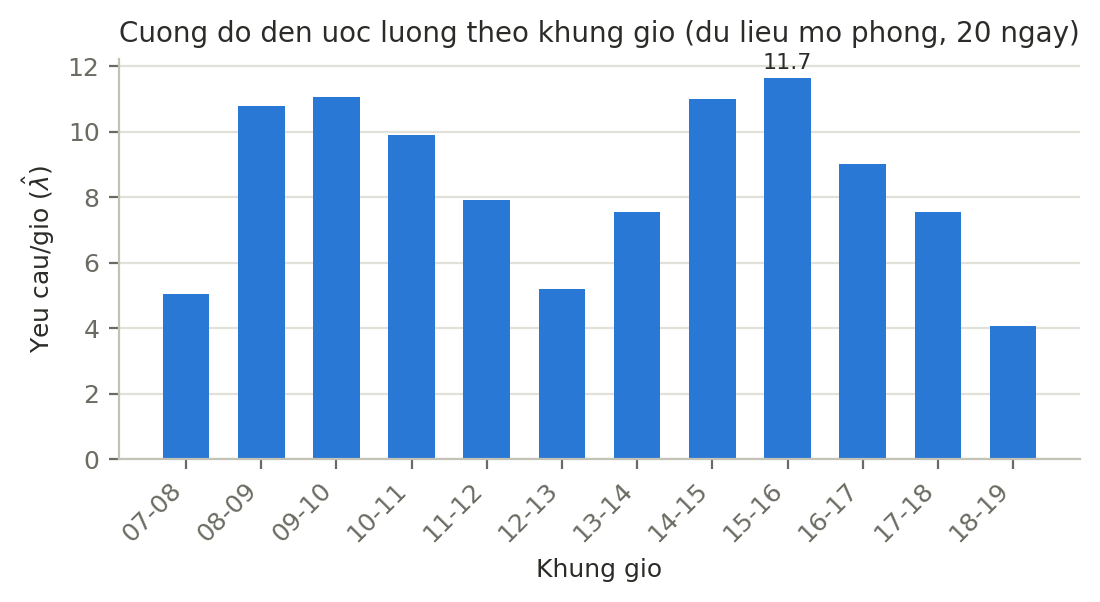
\includegraphics[width=0.9\linewidth]{figures/fig_arrivals.png}
\caption{Lượt xe đến theo khung giờ trong dữ liệu mô phỏng.}\label{r2:arrivals}
\source{\texttt{analysis/run\_analysis.py}; dữ liệu mô phỏng}
\end{figure}
\resulttable{tab_lambda.tex}{Lượt xe đến theo giờ và tham số sinh dữ liệu}{r2:lambda}
\FloatBarrier

\subsection{Đối chiếu công thức và mô phỏng}
\resulttable{tab_validation.tex}{Đối chiếu M/M/c với mô phỏng CV = 1, một loại xe, FCFS, 40 ngày/cấu hình, không bỏ đi}{r2:validation}
Ở $\rho\le0{,}84$, sai lệch nằm trong khoảng $-7{,}4\%$ đến $+7{,}5\%$. Ở
$\rho=0{,}98$ ($\lambda=225$, $c=6$) công thức cho 12,17 phút còn mô phỏng
7,61 phút ($-37{,}5\%$): khi gần bão hòa, mỗi ngày bắt đầu với hàng rỗng và
một giờ không đủ để hệ đạt trạng thái ổn định. Cấu hình $\lambda=212$, $c=5$
có $\rho=1{,}11$, không ổn định. Do đó M/M/c chỉ dùng để chọn công suất; kết
luận về phương án dựa trên mô phỏng.

\subsection{Điểm nghẽn AS-IS}
\resulttable{tab_asis_hourly.tex}{M/M/c theo giờ với 6 kênh và $E[S]=1{,}57$ phút}{r2:hourly}
\begin{figure}[htbp]\centering
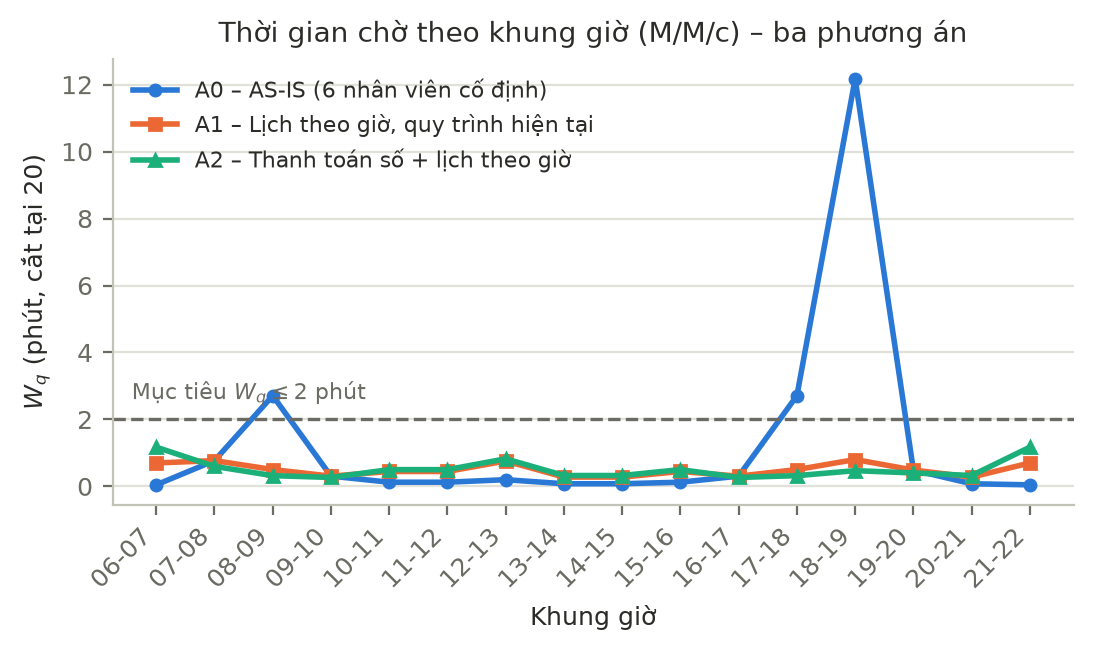
\includegraphics[width=0.89\linewidth]{figures/fig_wq_by_hour.png}
\caption{Thời gian chờ M/M/c theo giờ của ba phương án.}\label{r2:wq-hour}
\source{\texttt{analysis/run\_analysis.py}; tham số Bảng~\ref{r2:assumptions}}
\end{figure}
Lịch cố định 6 nhân viên vừa \emph{thừa} vừa \emph{thiếu}. Từ 09:00 đến 17:00,
$\rho$ chỉ 0,54--0,71; trong khi giờ 18--19 có $\rho=0{,}98$, $E[W_q]=12{,}17$
phút và 64\% xe chờ quá 5 phút; hai giờ 08--09 và 17--18 cũng vượt mục tiêu
(18,3\% chờ quá 5 phút). Mô phỏng cả ngày cho kết quả trung bình ``đẹp'' ---
$\overline{W_q}=0{,}64$ phút, mức sử dụng 67,9\% --- nhưng trong giờ 17--19
có 6,2\% xe chờ quá 5 phút và 2,3\% xe bỏ đi. Chẩn đoán vì vậy phải xét theo
giờ, không theo trung bình ngày.
\todo{2}{Thay $\lambda_t$ giả định bằng số hóa đơn điện tử theo giờ của một cửa
hàng thật (tối thiểu 4 tuần) và chạy lại toàn bộ.}

\section{Mô hình mở rộng: định vị rời rạc và dự báo nhu cầu}
\label{r2:extension}
\subsection{Chọn 2 trong 5 điểm mở cửa hàng mới}
\label{r2:location}
\textbf{Bài toán.} Doanh nghiệp có ngân sách mở $k=2$ cửa hàng mới và đã khảo
sát 5 vị trí ứng viên $J$ trên các trục chính; nhu cầu đến từ 8 quận $I$.
Bài toán định vị phân bố được rời rạc hóa bằng hai tập này. Dân số lấy theo
Tổng điều tra 2019~\cite{census2019}; nhu cầu mà một cửa hàng mới có thể thu
hút ở vùng $i$ là
\begin{equation}
h_i=\text{dân số}_i\times0{,}695\ \tfrac{\text{xe}}{\text{người}}\times0{,}2\
\tfrac{\text{lượt}}{\text{xe}\cdot\text{ngày}}\times2\%\ \text{(thị phần)},
\end{equation}
với 0,695 = 5,6 triệu xe máy / 8,05 triệu dân (E), 0,2 lượt/ngày = đổ 2,5 lít
mỗi 5 ngày (E), thị phần 2\% (G). Thời gian đi lại $t_{ij}$ (phút) tính từ tọa
độ xấp xỉ: khoảng cách đường chim bay $\times1{,}35$ (hệ số đường vòng), tốc
độ 20~km/giờ giờ cao điểm, cộng 2 phút ra/vào. Ngưỡng tiếp cận $R=15$ phút.
Năng lực một cửa hàng 8 vòi là $Q_j=2\,889$ lượt/ngày: giờ cao điểm (9\% lượt
ngày) tối đa 260 xe/giờ để vẫn đạt $\rho\le0{,}85$, $W_q\le2$ phút. Chi phí cố
định $f_j$ (thuê đất, khấu hao, quản lý) là 120, 150, 80, 95, 75 triệu đồng/tháng
cho J1--J5 (G). Mỗi lượt đóng góp $3{,}24\times1\,500-2\,165\approx2\,700$ đồng
(lãi gộp trừ lương nhân viên theo lượt).

\textbf{Mô hình.} $a_{ij}=1$ nếu $t_{ij}\le R$ (mã hóa nhị phân); vùng $i$ được
phủ khi tồn tại $j$ có $a_{ij}=1$ và $y_j=1$. Quyết định mở điểm được tích hợp
với phân bổ nhu cầu, chỉ giao cho điểm đã mở và không vượt năng lực:
\begin{align}
\text{(a)}\ \max\ \textstyle\sum_i h_i z_i \quad\text{hoặc}\quad
\text{(b)}\ \max\ 30\cdot2\,700\textstyle\sum_i h_i z_i/10^6-\sum_j f_j y_j \label{r2:mclp}\\
\text{với}\ \textstyle\sum_j y_j=2,\ x_{ij}\le a_{ij}y_j,\ \sum_j x_{ij}=z_i\le1,\
\sum_i h_i x_{ij}\le Q_j y_j,\ x,y,z\in\{0,1\}. \nonumber
\end{align}
Mục tiêu (a) là phục vụ được nhiều người nhất; mục tiêu (b) là lợi nhuận
(triệu đồng/tháng). Với $\binom52=10$ tổ hợp, nhóm liệt kê toàn bộ cách giao
vùng nên nghiệm là tối ưu chính xác.
\exttable{tab_ext_cover_matrix.tex}{Dân số, nhu cầu $h_i$ và thời gian đi lại $t_{ij}$ (phút); $^{\bullet}$ đánh dấu $a_{ij}=1$ ($t_{ij}\le15$ phút)}{r2:cover}
\exttable{tab_ext_location.tex}{Mười tổ hợp 2/5 điểm, xếp theo mục tiêu (a); lợi nhuận theo mục tiêu (b)}{r2:loc-result}
\begin{figure}[htbp]\centering
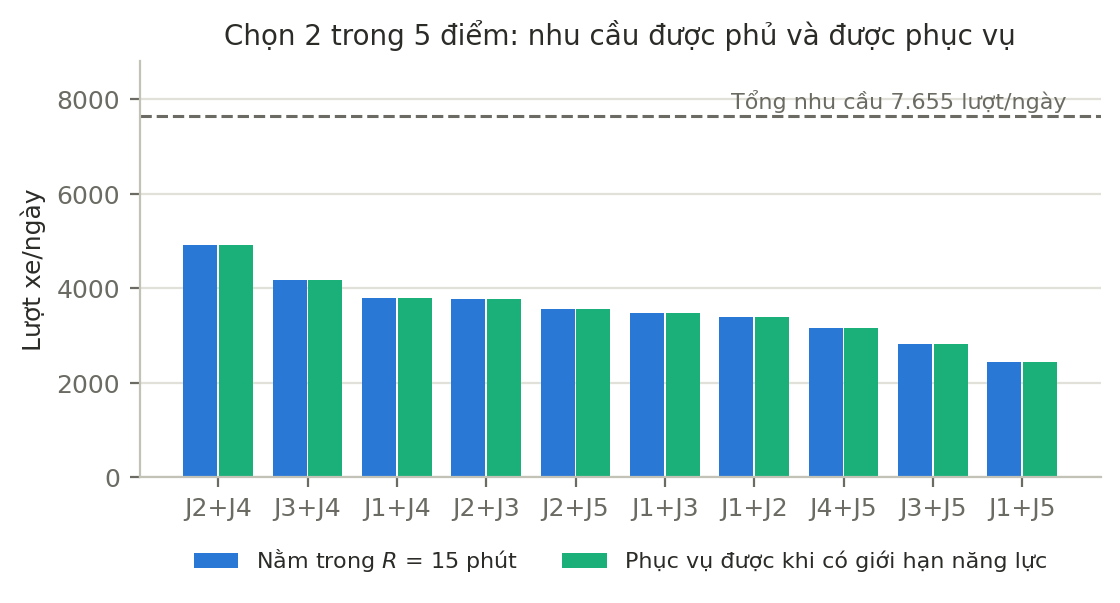
\includegraphics[width=0.9\linewidth]{figures/r2_location.png}
\caption{Nhu cầu nằm trong ngưỡng $R$ và nhu cầu phục vụ được của mười tổ hợp.}
\label{r2:loc-fig}
\source{\texttt{analysis/extension\_analysis.py}; dân số 2019, các tham số còn lại là ước tính/giả định}
\end{figure}

\textbf{Hai mục tiêu cho hai câu trả lời.} Theo mục tiêu (a), \textbf{J2 Đống Đa +
J4 Hoàng Mai} phục vụ 4\,916 lượt/ngày (64,2\% nhu cầu); J2 nhận Cầu Giấy, Đống
Đa, Thanh Xuân (2\,664 lượt/ngày, $\rho_{\max}=0{,}78$). Theo mục tiêu (b),
\textbf{J3 Hà Đông + J4 Hoàng Mai} lãi 163,2 triệu đồng/tháng so với 153,2 triệu
của J2 + J4, dù chỉ phục vụ 54,5\% nhu cầu: J2 nằm ở vùng giá thuê cao
(150 triệu đồng/tháng) và phải gánh tải gần năng lực. Một doanh nghiệp tư nhân
chịu áp lực chiết khấu thấp sẽ chọn (b); nếu mục tiêu là độ phủ dịch vụ (ví
dụ cam kết với đầu mối về sản lượng), (a) phù hợp hơn.

\exttable{tab_ext_location_sens.tex}{Độ nhạy của quyết định định vị}{r2:loc-sens}
\textbf{Độ bền.} J3 + J4 là tổ hợp lãi nhất ở 5/6 tình huống: $R=15$ hoặc 20
phút, nhu cầu giảm 20\% (KB-A), tăng 20\% (KB-B) và cửa hàng chỉ có 6 vòi; khi
nhu cầu tăng 20\%, J3 + J4 còn trở thành phương án phục vụ nhiều nhất vì J2 bị
giới hạn năng lực. Ngược lại, lợi nhuận của J2 + J4 giảm còn 73,6 triệu khi
nhu cầu giảm 20\% và còn 18,9 triệu nếu chỉ có 6 vòi. Chỉ khi $R=12$ phút (khách
rất ngại đi xa) thì tối ưu lợi nhuận chuyển sang J4 + J5. Kết luận BT2:
\textbf{chọn J3 Hà Đông + J4 Hoàng Mai}, giữ J4 cố định và coi J2/J3 là lựa
chọn phụ thuộc mục tiêu.
\todo{2}{Thay tọa độ xấp xỉ bằng địa chỉ ứng viên thật và thời gian đi lại từ
bản đồ số; kiểm tra lại số cửa hàng đối thủ trong bán kính $R$ để hiệu chỉnh thị phần 2\%.}

\subsection{Dự báo lượt xe ngày tới bằng học máy}
\label{r2:forecast}
Lịch theo giờ (BT1) chỉ tốt khi biết trước $\lambda_t$. Nhu cầu xăng có các
biến động \emph{biết trước được}: giá điều chỉnh vào 15 giờ thứ Năm hằng tuần
(tăng giá thì khách đổ trước 15 giờ, giảm giá thì chờ sau 15 giờ), tuần trước
Tết và kỳ nghỉ Tết, và tín hiệu căng thẳng nguồn cung. Nhóm dựng lịch sử 2 năm
(25/11/2024--22/11/2026) với \emph{lịch sự kiện thật}: Tết Ất Tỵ 29/1/2025, Tết
Bính Ngọ 17/2/2026, đợt cửa hàng đóng cửa giữa 2025 và đợt 17 cửa hàng tạm
dừng bán đầu tháng 3/2026~\cite{vtc2026}; biên độ điều chỉnh giá theo tuần lấy
quanh mức của các kỳ gần đây (1\,310--2\,075 đồng/lít~\cite{moit2026}). Lượt xe
trong lịch sử là mô phỏng. Mô hình học máy là hồi quy Poisson (GLM, ước lượng IRLS):
\begin{multline}
\log\lambda_{d,h}=\beta_h+\gamma_{\text{thứ}(d)}+\delta_1\sin\tfrac{2\pi d}{364}+\delta_2\cos\tfrac{2\pi d}{364}
+\tau_1 T^{\text{trước}}_d+\tau_2 T^{\text{nghỉ}}_d\\
+\pi_1\Delta p_d\mathbf 1_{h<15}+\pi_2\Delta p_d\mathbf 1_{h\ge15}+\pi_3\Delta p_{d-1}+\eta s_{d-1}+\kappa\ell_{d-1},
\end{multline}
với $\Delta p_d$ là mức điều chỉnh dự kiến (nghìn đồng/lít, tính được trước từ
giá thế giới), $s_{d-1}$ là tín hiệu nguồn cung hôm trước, $\ell_{d-1}$ là log tỷ
số lượt hôm trước so với trung bình 28 ngày. Học trên 23/12/2024--4/1/2026,
kiểm tra trên 84 ngày 5/1--29/3/2026 (có Tết và đợt tháng 3).
\exttable{tab_ext_ml_acc.tex}{Độ chính xác dự báo trên 84 ngày kiểm tra; ``ngày sự kiện'' là 25 ngày có Tết, điều chỉnh giá $\ge$1\,000 đồng/lít hoặc căng thẳng nguồn cung}{r2:ml-acc}
\begin{figure}[htbp]\centering
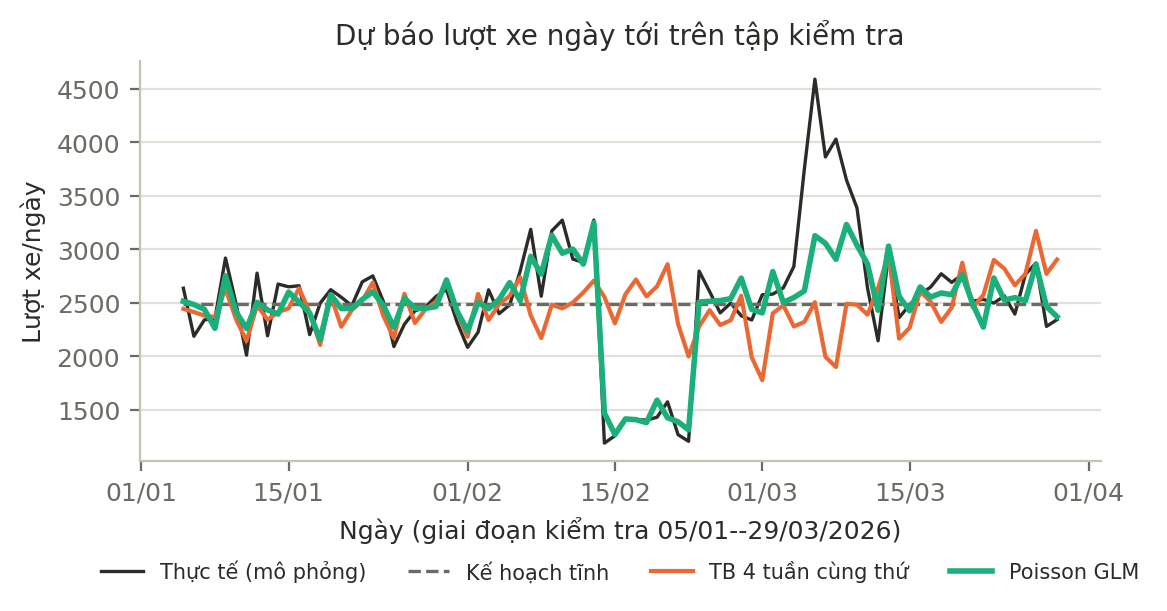
\includegraphics[width=0.9\linewidth]{figures/r2_forecast.png}
\caption{Dự báo tổng lượt xe/ngày trên tập kiểm tra.}\label{r2:ml-fig}
\source{\texttt{analysis/extension\_analysis.py}; lượt xe mô phỏng, lịch sự kiện theo thực tế}
\end{figure}
GLM giảm MAPE tổng ngày từ 18,33\% (kế hoạch tĩnh) và 19,63\% (trung bình 4 tuần
cùng thứ) xuống 7,25\%; trên 25 ngày sự kiện, từ khoảng 46\% xuống 10,44\%.
Trung bình 4 tuần thậm chí kém kế hoạch tĩnh vì nó ``nhớ'' Tết và đợt tháng 3
sang các tuần sau (Hình~\ref{r2:ml-fig}). Hệ số ước lượng có ý nghĩa vận hành:
tuần trước Tết $+18\%$ ($e^{0{,}167}$), kỳ nghỉ Tết $-42\%$ ($e^{-0{,}540}$), mỗi
nghìn đồng/lít tăng giá làm lượt xe trước 15 giờ tăng 28\% ($e^{0{,}249}$).
Giá trị vận hành của dự báo được đánh giá ở Mục~\ref{r3:ml-staff}.
\todo{2}{Huấn luyện lại trên dữ liệu hóa đơn điện tử thật; giữ cách chia theo
thời gian (không trộn ngẫu nhiên) và báo cáo MAPE theo tháng.}

\FloatBarrier
\clearpage
% !TeX root = _main.tex
% ROLE 3 -- TO-BE, DANH GIA, KICH BAN CHIEN LUOC, TRAI NGHIEM KHACH HANG, KET LUAN (muc 8--11).
% Nguoi nhan: nhom tu dien. Muc tieu: 6--8 trang noi dung chinh.
% DUOC SUA: file nay, figures/r3_*; nhan \label bat dau bang r3:.
% KHONG SUA: role_1.tex, role_2.tex, cac file dieu phoi; thong nhat voi role 2
% truoc khi thay du lieu analysis/. Khong sua tay bang sinh tu Python.
% DAU VAO: tables/tab_{comparison,shift_plan,sensitivity,risk}.tex, tables/tab_ext_*.tex.

\section{Phương án cải tiến và phân bổ nhân lực}
\label{r3:tobe}
\subsection{Ba phương án đối chứng}
\begin{table}[htbp]\centering\small
\caption{Thiết kế các phương án trong so sánh mô phỏng}\label{r3:scenarios-design}
\begin{tabularx}{\linewidth}{@{}p{26mm}Y Y Y@{}}
\toprule
Thành phần & A0: AS-IS & A1: lịch theo giờ & A2: số hóa + lịch \\
\midrule
Số kênh $c_t$ & 6 cả ngày & Tối ưu BT1 với $E[S]$ hiện tại & Tối ưu BT1 với $E[S]$ TO-BE \\
$E[S]$ (phút/xe) & xe máy 1,5; ô tô 4,0 & như A0 & giảm 20\%: 1,2; 3,2 \\
Thanh toán & Tiền mặt/QR tại trụ & như A0 & Trả trước QR/ứng dụng, chọn sẵn số tiền \\
Giờ nhân viên/ngày & 96 & 88 & 72 \\
Mục đích & Mốc hiện trạng & Tác động riêng của lịch & Tác động kết hợp lịch + số hóa \\
\bottomrule
\end{tabularx}
\end{table}
So sánh A0--A1 tách được tác động của việc xếp lịch theo giờ; so sánh A1--A2
tách được tác động của số hóa thanh toán (với lịch được tối ưu lại tương ứng).

\subsection{Bài toán lập lịch theo giờ (BT1)}
Với $k=58\,000$ đồng/giờ nhân viên và 16 khung một giờ:
\begin{align}
\min_{c_1,\ldots,c_{16}}\quad & k\textstyle\sum_{t=1}^{16}c_t \\
\text{với}\quad & c_t\in\{1,\ldots,8\},\ \rho_t<1,\ E[W_{q,t}]\le2\text{ phút},\ P(W_{q,t}>5)\le0{,}05. \nonumber
\end{align}
Chi phí cộng theo giờ và ràng buộc tách theo giờ, nên chọn $c_t$ nhỏ nhất khả thi
cho từng giờ là tối ưu trong mô hình. Đây là kế hoạch công suất; lịch ca cá
nhân (ca 4--8 giờ, nghỉ giữa ca) cần thêm một bước ghép ca.
\resulttable{tab_shift_plan.tex}{Số kênh theo giờ của ba phương án}{r3:staffing}
\begin{figure}[htbp]\centering
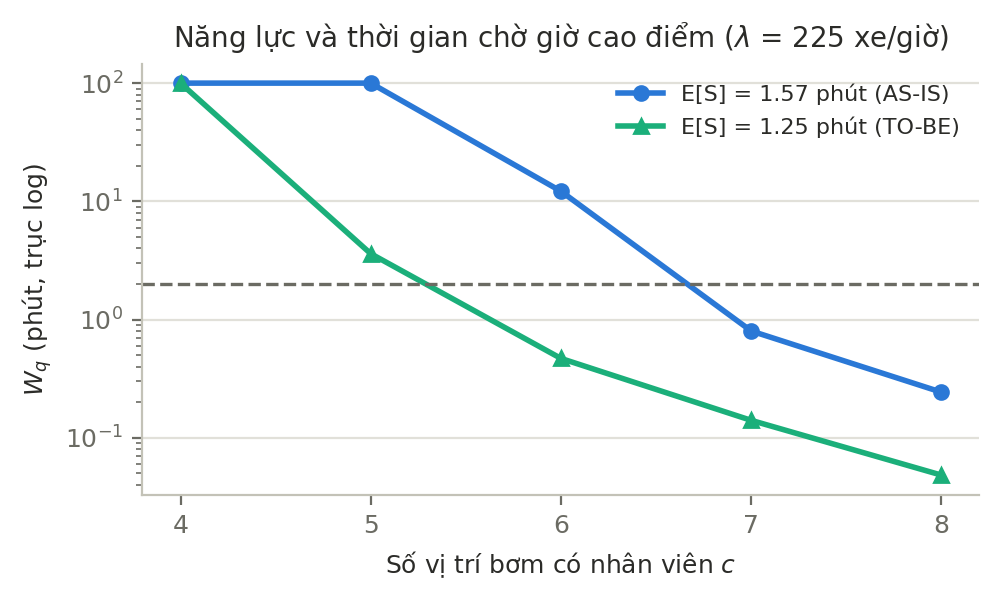
\includegraphics[width=0.82\linewidth]{figures/fig_wq_vs_c.png}
\caption{Thời gian chờ giờ cao điểm theo số kênh (M/M/c).}\label{r3:wq-c}
\source{\texttt{analysis/run\_analysis.py}; tham số Bảng~\ref{r2:assumptions}}
\end{figure}
A1 dồn nhân viên vào 07--09 và 16--19 (6--7 kênh) và rút về 4--5 kênh lúc vắng;
tổng giảm từ 96 xuống 88 giờ/ngày nhưng giờ cao điểm lại nhiều kênh hơn A0.
A2 cần 72 giờ/ngày vì mỗi kênh phục vụ được 47,8 thay vì 38,3 xe/giờ.

\subsection{Quy trình TO-BE}
\begin{figure}[htbp]\centering
\resizebox{\linewidth}{!}{%
\begin{tikzpicture}
\def\W{18.4}
\foreach \y/\name in {0/Khách hàng,-2.4/Nhân viên bơm,-4.8/Ứng dụng / POS / HĐĐT}{
  \draw (0,\y) rectangle (\W,\y-2.4);
  \draw (0.8,\y) -- (0.8,\y-2.4);
  \node[rotate=90,font=\scriptsize\bfseries] at (0.4,\y-1.2) {\name};}
\node[ev] (st) at (1.6,-1.2) {};
\node[task] (t0) at (3.4,-1.2) {Chọn số tiền,\\trả trước QR};
\node[task] (s0) at (3.4,-6.0) {Tạo mã đơn,\\hiển thị ETA};
\node[gw] (g1) at (6.0,-1.2) {Hàng chờ\\$\ge$ 20 xe?};
\node[evend] (eb) at (7.7,-0.45) {};
\node[font=\scriptsize,anchor=west] at (8.1,-0.45) {bỏ đi};
\node[task] (t2) at (8.8,-1.6) {Xếp hàng\\chờ tới lượt};
\node[task] (t3) at (11.2,-3.6) {Quét mã,\\bơm đúng số tiền};
\node[task] (s1) at (13.6,-6.0) {HĐĐT tự động\\gửi về ứng dụng};
\node[task] (t7) at (15.8,-1.2) {Rời trụ\\(không thu tiền)};
\node[evend] (en) at (17.7,-1.2) {};
\node[task,dashed] (pl) at (8.8,-6.0) {Lịch $c_t$ theo\\dự báo (BT1 + GLM)};
\draw[flow] (st) -- (t0);
\draw[msg] (t0) -- (s0);
\draw[flow] (t0) -- (g1);
\draw[flow] (g1.north) |- node[pos=0.25,left,font=\scriptsize]{có} (eb);
\draw[flow] (g1.east) -- node[above,font=\scriptsize]{không} ++(0.6,0) |- (t2);
\draw[flow] (t2) |- (t3);
\draw[flow] (t3) -| (s1);
\draw[flow] (s1) -| (t7);
\draw[flow] (t7) -- (en);
\draw[msg] (pl) -| (t3);
\node[tmark] at (11.2,-4.35) {$S$ giảm 20\%: không thu tiền mặt};
\end{tikzpicture}}
\caption{Quy trình TO-BE: thanh toán trước khi vào trụ, hóa đơn tự động, số nhân viên theo dự báo. Khách không dùng ứng dụng vẫn đi theo luồng AS-IS ở Hình~\ref{r1:bpmn}.}
\label{r3:bpmn}
\source{nhóm vẽ bằng TikZ theo ký pháp BPMN rút gọn; Claude Code hỗ trợ dựng mã hình}
\end{figure}
Thay đổi chính là đưa thanh toán và xuất hóa đơn ra khỏi thời gian chiếm trụ.
Kênh tiền mặt vẫn giữ cho khách lớn tuổi (Mục~\ref{r3:cx}); nếu tỷ lệ khách
dùng trả trước thấp, mức giảm $E[S]$ sẽ nhỏ hơn 20\% (rủi ro ở Bảng~\ref{r3:risks}).
\FloatBarrier

\section{Đánh giá, độ nhạy và giới hạn}
\label{r3:evaluation}
\subsection{So sánh trên cùng bộ chỉ số}
\resulttable{tab_comparison.tex}{Kết quả mô phỏng chính: 20 ngày, cùng seed, CV = 0,8}{r3:comparison}
\begin{itemize}
\item \textbf{Lịch theo giờ (A1) giải quyết phần lớn vấn đề mà không cần đầu tư.}
Trong giờ 17--19, tỷ lệ chờ quá 5 phút giảm từ 6,18\% xuống 0,50\%, tỷ lệ bỏ đi
từ 2,26\% xuống 0,17\%, đồng thời giảm 8 giờ nhân viên/ngày (464 nghìn đồng/ngày).
\item \textbf{Số hóa (A2) chủ yếu tiết kiệm nhân lực.} Thời gian chờ chỉ giảm
thêm ít (0,45 $\rightarrow$ 0,43 phút cả ngày; 0,56 $\rightarrow$ 0,36 phút giờ
17--19), nhưng giảm thêm 16 giờ/ngày. Sau khi trừ 250 nghìn đồng/ngày chi phí số
hóa, A2 rẻ hơn A1 678 nghìn đồng/ngày và rẻ hơn A0 1,14 triệu đồng/ngày
(khoảng 34 triệu đồng/tháng).
\item Ô tô và xe máy dùng chung hàng nên thời gian chờ gần như nhau (A0: 0,59
và 0,64 phút); ô tô chỉ làm tăng $E[S]$ bình quân.
\end{itemize}
\begin{figure}[htbp]\centering
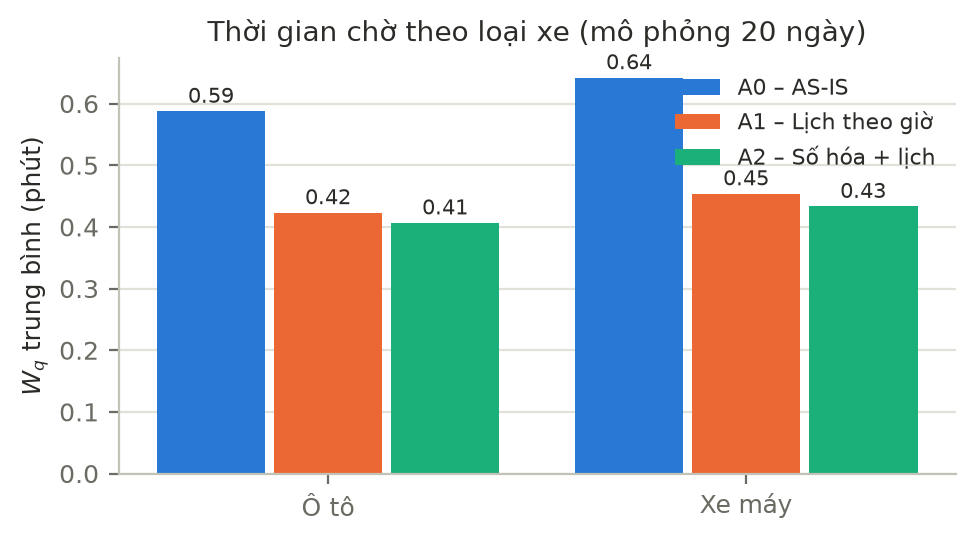
\includegraphics[width=0.82\linewidth]{figures/fig_by_class.png}
\caption{Thời gian chờ theo loại xe của ba phương án.}\label{r3:by-class}
\source{\texttt{analysis/run\_analysis.py}; dữ liệu mô phỏng}
\end{figure}
\FloatBarrier

\subsection{Độ nhạy theo nhu cầu}
\resulttable{tab_sensitivity.tex}{Độ nhạy theo hệ số nhu cầu (30 ngày, seed riêng, giữ nguyên lịch)}{r3:sensitivity}
\begin{figure}[htbp]\centering
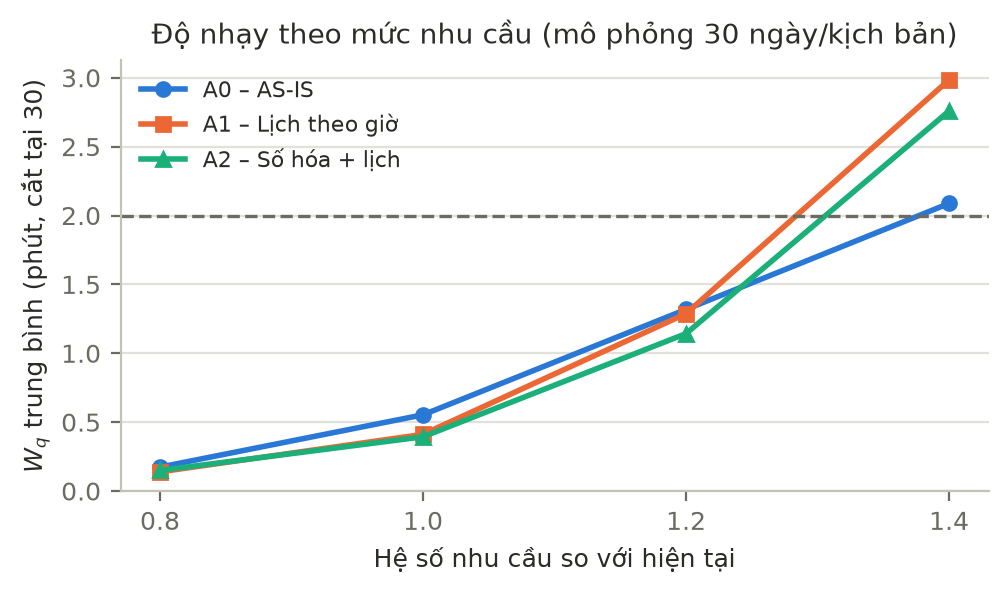
\includegraphics[width=0.85\linewidth]{figures/fig_sensitivity.png}
\caption{Thời gian chờ trung bình khi nhu cầu thay đổi, giữ nguyên lịch.}\label{r3:sens-fig}
\source{\texttt{analysis/run\_analysis.py}; 30 ngày mô phỏng mỗi cấu hình}
\end{figure}
Khi nhu cầu tăng 20\%, cả ba lịch \emph{giữ nguyên} đều có $\rho$ giờ cao điểm
gần hoặc vượt 1; A2 vẫn đạt $P(W_q{>}5)=2{,}61\%$ nhưng 0,53\% khách bỏ đi.
Khi tăng 40\%, mọi lịch đều hỏng (4,9--7,9\% khách bỏ đi). Một lịch tĩnh, dù
tối ưu cho tải cơ sở, không bền trước biến động nhu cầu --- đây là lý do của
BT3 và BT4 ở Mục~\ref{r3:scenarios}.

\subsection{Rủi ro và giới hạn}
\resulttable{tab_risk.tex}{Các tình huống rủi ro của A2 (30 ngày, seed riêng)}{r3:risks}
Thiếu một nhân viên ở mọi giờ làm $P(W_q{>}5)$ tăng lên 16,80\% và 1,93\% khách
bỏ đi: A2 tiết kiệm nhân lực nên ít dư địa. Nếu số hóa chỉ giảm 10\% thời gian
phục vụ, A2 vẫn đạt mục tiêu (1,45\%; 0,10\% bỏ đi). Các giới hạn cần giữ:
\begin{itemize}
\item Lượt xe theo giờ và thời gian phục vụ là mô phỏng; quy mô được hiệu chỉnh
từ số liệu công bố nhưng chưa đo tại một cửa hàng cụ thể.
\item Mô hình coi mọi vòi phục vụ mọi loại xe; thực tế có trụ riêng cho ô tô.
\item Ngưỡng bỏ đi 20 xe và các tham số trải nghiệm khách hàng là giả định.
\item Mỗi ngày bắt đầu với hàng rỗng; kiểm chứng ở tải rất cao còn lệch (Mục~\ref{r2:diagnosis}).
\end{itemize}

\section{Kịch bản chiến lược và trải nghiệm khách hàng}
\label{r3:scenarios}
\subsection{Ba kịch bản tương lai và hai lựa chọn chiến lược}
Từ PESTEL (Bảng~\ref{r1:pestel}), nhóm xây ba kịch bản cho cửa hàng ở tầm
12--24 tháng. Xác suất chỉ dùng để tính chi phí kỳ vọng; tiêu chí chính là
hối tiếc tối đa, không phụ thuộc xác suất.
\begin{itemize}
\item \textbf{KB-A -- Nhu cầu thấp} (0,30): lượt xe $\times0{,}8$ do vùng phát
thải thấp mở rộng và khách chuyển sang xe điện~\cite{ct20,lez2026}.
\item \textbf{KB-B -- Nhu cầu tăng} (0,45): lượt xe $\times1{,}2$ do cửa hàng lân
cận đóng cửa vì chiết khấu thấp~\cite{chietkhau} và xe máy mới tăng~\cite{reg2025}.
\item \textbf{KB-C -- Gián đoạn} (0,25): như đợt tháng 3/2026~\cite{vtc2026},
khách dồn sang ($\times1{,}35$) và bán có kiểm soát làm thời gian phục vụ tăng 15\%.
\end{itemize}
Lựa chọn \textbf{CL-A -- nhân lực theo lịch, không số hóa} giữ lịch A1 (88 giờ).
Lựa chọn \textbf{CL-B -- số hóa} có hai biến thể: \emph{tĩnh} giữ lịch A2 (72 giờ);
\emph{thích ứng} dùng dự báo (Mục~\ref{r2:forecast}) để tối ưu lại $c_t$ theo
BT1 mỗi ngày, phần giờ vượt lịch A2 do nhân viên bán thời gian đảm nhận với đơn
giá $1{,}5\times58\,000$ đồng/giờ. Mỗi ô mô phỏng 30 ngày, cùng seed trong một
kịch bản.

\subsection{Mô hình mất khách theo thế hệ}
\label{r3:cx}
Mục tiêu dài hạn của chiến lược là khách quay lại, không bỏ cửa hàng. Một khách
thuộc phân khúc $g$ đã chờ $w$ phút có xác suất không hài lòng đến mức lần sau
bỏ đi là
\begin{equation}
p_g(w)=1-\exp\!\left[-(w/\theta_g)^2\right],
\end{equation}
dạng Weibull để chờ ngắn gần như không gây mất khách còn chờ dài làm xác suất
tăng nhanh; khách bỏ đi vì hàng dài có $p=1$. Mỗi lượt mất gây thiệt hại
$p\times[\text{lãi gộp lượt đó}+c_g\times\text{CLV}]$, với $c_g$ là xác suất
chuyển hẳn sang cửa hàng khác. CLV là lãi gộp 3 năm của một khách quen: xe máy
$73\times2{,}5\times1\,500\times3\approx820$ nghìn đồng, ô tô
$52\times30\times1\,500\times3\approx7{,}02$ triệu đồng. Các giá trị $\theta_g$,
$c_g$ trong Bảng~\ref{r3:segments} là giả định để thể hiện cơ chế, chưa có khảo sát.
\exttable{tab_ext_segments.tex}{Tỷ lệ mất khách theo phân khúc trong KB-B; $\theta_g$, $c_g$ là giả định}{r3:segments}
\textbf{Nhận định.} Với cùng một hàng chờ, Gen Z mất 8,79\% ở A0 so với 4,77\%
ở nhóm 60+. Khi chờ đã ngắn (CL-B thích ứng), khoảng cách tương đối còn lớn
hơn (1,41\% so với 0,50\%, gấp 2,8 lần): nhóm trẻ --- nhiều người là sinh viên
và tài xế giao hàng --- là nhóm đầu tiên rời đi và cũng là nhóm chuyển sang xe
điện sớm nhất. Hàm ý: thông báo thời gian chờ dự kiến và trả trước trên ứng
dụng cho nhóm trẻ; giữ thu tiền mặt và nhân viên hỗ trợ cho nhóm lớn tuổi.

\subsection{Kết quả theo kịch bản}
\exttable{tab_ext_scenarios.tex}{Hiệu quả của các chiến lược trong ba kịch bản; chi phí và giá trị mất tính bằng nghìn đồng/ngày}{r3:scen-table}
\begin{figure}[htbp]\centering
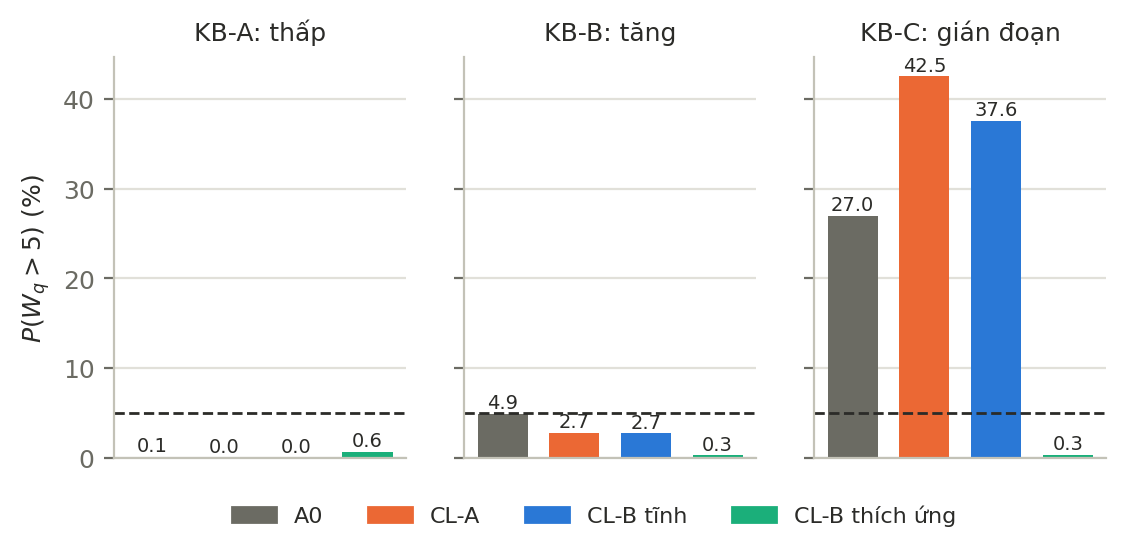
\includegraphics[width=0.92\linewidth]{figures/r3_scenarios.png}
\caption{Tỷ lệ xe chờ quá 5 phút theo kịch bản; đường đứt là mục tiêu 5\%.}
\label{r3:scen-fig}
\source{\texttt{analysis/extension\_analysis.py}; dữ liệu mô phỏng}
\end{figure}
(1) Ở KB-A mọi lựa chọn đều đạt; CL-B tĩnh rẻ nhất (4,68 triệu đồng/ngày) vì
biến thể thích ứng cắt xuống 59 giờ và làm chờ tăng nhẹ. (2) Ở KB-B, lịch tĩnh
vẫn đạt $P(W_q{>}5)\le5\%$ nhưng 3,6--4,4\% khách bị mất; CL-B thích ứng tăng lên
81 giờ và chỉ mất 0,98\%. (3) KB-C quyết định lựa chọn: mọi lịch tĩnh đều sụp
(37,6--42,5\% xe chờ quá 5 phút, 11,8--13,6\% bỏ đi), trong khi CL-B thích ứng
giữ 0,30\% với 101 giờ/ngày --- gần chạm giới hạn 8 vòi ở giờ cao điểm.
\exttable{tab_ext_regret.tex}{Tổng chi phí (nghìn đồng/ngày), kỳ vọng và hối tiếc tối đa; ``đạt'' khi $P(W_q{>}5)\le5\%$ và bỏ đi $\le1\%$}{r3:regret}

\subsection{Đánh giá và quyết định}
Nhóm chọn \textbf{CL-B thích ứng}: hối tiếc tối đa chỉ 554,8 nghìn đồng/ngày
(ở KB-A) so với 59--66 triệu đồng/ngày của hai lựa chọn tĩnh (ở KB-C); chi phí kỳ
vọng 7,31 so với 23,90--26,72 triệu đồng/ngày; và là lựa chọn duy nhất đạt mục
tiêu ở cả ba kịch bản.
\exttable{tab_ext_clv.tex}{Chi phí kỳ vọng (nghìn đồng/ngày) theo hệ số CLV}{r3:clv}
\textbf{Kết luận có bền không?} Ngay cả khi bỏ hoàn toàn giá trị khách quay lại
(CLV = 0, chỉ tính lãi gộp của lượt bị mất), CL-B thích ứng vẫn rẻ nhất
(5,34 so với 5,87 và 6,71 triệu đồng/ngày) vì khách bỏ đi trong KB-C là doanh
thu mất ngay. Điều kiện để kết luận đúng là \emph{dự báo đủ tốt} và \emph{có
nguồn nhân viên bán thời gian huy động được trong ngày}.

\subsection{Năng lực thích ứng nhờ dự báo}
\label{r3:ml-staff}
Mô hình GLM ở Mục~\ref{r2:forecast} được dùng để lập lịch $c_t$ cho từng ngày
kiểm tra; mỗi ngày được mô phỏng với nhu cầu thật của ngày đó.
\exttable{tab_ext_ml_staff.tex}{Lập lịch theo dự báo trên 84 ngày kiểm tra (5/1--29/3/2026); ngày vi phạm: $P(W_q{>}5)>5\%$ hoặc bỏ đi $>1\%$}{r3:ml-staff-table}
Lịch A2 tĩnh vi phạm ở 16,7\% số ngày và 10,67\% xe chờ quá 5 phút trong các
ngày sự kiện. Lịch theo GLM giảm số ngày vi phạm xuống 6,0\% mà chỉ dùng 70,48
giờ/ngày --- ít hơn lịch tĩnh. Phương án ``đệm 20\%'' đạt kết quả tương đương
(7,1\% ngày vi phạm) nhưng tốn 81 giờ/ngày; GLM tiết kiệm 10,5 giờ, tức 610
nghìn đồng/ngày (khoảng 18 triệu đồng/tháng). Lịch theo trung bình 4 tuần còn
kém lịch tĩnh (27,4\% ngày vi phạm) vì phản ứng trễ với sự kiện.

\begin{table}[htbp]\centering\small
\caption{Kế hoạch ứng phó: dấu hiệu sớm, ngưỡng kích hoạt và hành động}\label{r3:playbook}
\begin{tabularx}{\linewidth}{@{}p{14mm}Y Y Y@{}}
\toprule
Kịch bản & Dấu hiệu sớm & Ngưỡng kích hoạt & Hành động \\
\midrule
KB-A & Lượt xe dự báo giảm; vùng phát thải thấp mở rộng & $<2\,000$ lượt/ngày trong 4 tuần & Giảm kênh lúc vắng; đàm phán lắp tủ đổi pin/trạm sạc~\cite{vgx} \\
KB-B & Cửa hàng lân cận đóng cửa; dự báo tăng & $>2\,900$ lượt/ngày hoặc $\rho_{17-19}>0{,}85$ & Tối ưu lại $c_t$ ($\approx$81 giờ/ngày); tuyển thêm nhân viên bán thời gian \\
KB-C & Tin căng thẳng nguồn cung; điều chỉnh giá lớn & Tín hiệu nguồn cung hoặc $|\Delta p|\ge1\,000$ đồng/lít & Mở đủ 8 vòi giờ cao điểm; gọi ca dự phòng; hiển thị ETA, ưu tiên khách trả trước \\
\bottomrule
\end{tabularx}
\end{table}

\begin{table}[htbp]\centering\small
\caption{Học máy trong dịch vụ: tác động, chỉ số chấp nhận và kiểm soát}\label{r3:ml-uses}
\begin{tabularx}{\linewidth}{@{}p{27mm}Y Y Y@{}}
\toprule
Ứng dụng & Tác động lên mô hình & Chỉ số chấp nhận & Kiểm soát \\
\midrule
Dự báo lượt xe (đã thử) & $\hat\lambda_{d,h}\to c_t$ & MAPE $\le10\%$; ngày vi phạm $\le7\%$ & Cửa hàng trưởng duyệt lịch hằng ngày \\
Ước lượng độ kiên nhẫn & $\theta_g$ từ tỷ lệ bỏ đi theo độ dài hàng & Sai số dự báo bỏ đi & Chỉ dùng dữ liệu ẩn danh, gộp \\
Dự báo rời bỏ & Khách quen giảm tần suất & AUC; tỷ lệ giữ chân & Ưu đãi có đồng ý của khách \\
Phát hiện bất thường & Lượt bán đột biến, lỗi cột bơm & Thời gian phát hiện & Kiểm tra thủ công trước khi xử lý \\
\bottomrule
\end{tabularx}
\end{table}

\section{Kết luận và đề xuất định hướng}
\label{r3:conclusion}
Trong bộ giả định đã hiệu chỉnh theo số liệu công bố, vấn đề của cửa hàng đại
diện không phải thiếu nhân viên mà là \emph{nhân viên đặt sai giờ}: lịch cố định
6 người thừa công suất ban ngày nhưng để 6,2\% xe chờ quá 5 phút và 2,3\% xe bỏ
đi giờ tan tầm. Trung bình cả ngày (0,64 phút) che khuất điểm nghẽn này.

\textbf{Đề xuất.} Nhóm đề xuất chiến lược \textbf{``số hóa có lịch thích ứng''
(CL-B thích ứng)}, triển khai ba bước:
\begin{enumerate}
\item \textbf{0--3 tháng -- Đo và xếp lại lịch.} Xuất dấu thời gian từ hóa đơn
điện tử theo giờ, bấm giờ 30--50 lượt mỗi loại xe; áp dụng ngay lịch theo giờ
(A1): giảm 8 giờ/ngày và đưa tỷ lệ bỏ đi giờ 17--19 từ 2,26\% về 0,17\% mà
không cần đầu tư.
\item \textbf{3--6 tháng -- Số hóa thanh toán.} Trả trước QR/ứng dụng và hóa
đơn tự động; khi $E[S]$ giảm 20\%, lịch còn 72 giờ/ngày, tiết kiệm khoảng 34
triệu đồng/tháng so với hiện trạng. Giữ kênh tiền mặt cho khách lớn tuổi.
\item \textbf{6--12 tháng -- Lịch thích ứng và mở rộng.} Dùng GLM dự báo lượt xe
ngày tới (MAPE 7,25\% trong kiểm tra), lập nhóm nhân viên bán thời gian cho
ngày sự kiện; khi mở cửa hàng mới, ưu tiên \textbf{J3 Hà Đông + J4 Hoàng Mai}
(lãi 163,2 triệu đồng/tháng, bền ở 5/6 tình huống độ nhạy) và chuẩn bị mặt
bằng cho đổi pin/sạc nếu KB-A xảy ra.
\end{enumerate}
Theo dõi bốn KPI theo tháng --- $P(W_q{>}5)$ giờ 17--19, tỷ lệ bỏ đi, tỷ lệ mất
khách theo nhóm tuổi, MAPE dự báo --- và xem lại chiến lược khi một ngưỡng ở
Bảng~\ref{r3:playbook} bị vượt. Các kết luận dựa trên mô phỏng; mức giảm $E[S]$,
ngưỡng bỏ đi, độ kiên nhẫn theo thế hệ và chi phí cố định phải được đo lại tại
cửa hàng thật trước khi triển khai.
\todo{3}{Đối chiếu từng con số trong mục này với \path{analysis/data/run_log.txt}
và \path{analysis/data/ext_run_log.txt} sau lần chạy cuối cùng.}

\FloatBarrier
\clearpage

\phantomsection
\addcontentsline{toc}{section}{Tài liệu tham khảo}
\begin{thebibliography}{9}
\bibitem{rubric} Học phần INT3501, \textit{Hướng dẫn dự án nhóm và rubric}.
Tài liệu nội bộ: \path{Lecture/INT3501_Huong_dan_du_an_Rubric.pdf}.
\bibitem{checkpoint2} Nhóm 8, \textit{Báo cáo Checkpoint 2: Smart Healthcare}, 2026.
Tệp PDF mẫu trong thư mục \texttt{CP\_Assigment/} của dự án.
\bibitem{analysis} Nhóm 8, \textit{Mã nguồn và kết quả phân tích hàng đợi}.
Các tệp \texttt{run\_analysis.py}, \texttt{simulate.py}, \texttt{queueing.py},
\path{data/run_log.txt} trong \path{Subbmittion/FinalProject/analysis/}.
\end{thebibliography}
% Them nguon hoc thuat SAU KHI da doc/kiem chung; khong tu dien DOI/nam/tac gia.

\appendix
\section{Phân công và cách ghép báo cáo}
\label{app:roles}
\begin{table}[H]\centering\small
\caption{Phạm vi làm việc song song; mỗi người nhận một role}
\begin{tabularx}{\linewidth}{@{}p{21mm}Y Y@{}}
\toprule
File & Nội dung chịu trách nhiệm & Đầu ra bàn giao \\
\midrule
\texttt{role\_1.tex} & Bài toán, khung hệ thống, Resource Map, Journey/Blueprint và BPMN AS-IS. & Mục 1--4, sơ đồ AS-IS, liên hệ điểm nghẽn với biến đo. \\
\texttt{role\_2.tex} & Dữ liệu, giả định, hàng đợi, mô phỏng, kiểm chứng và chẩn đoán AS-IS. & Mục 5--6, bảng tham số, kết quả và giới hạn kiểm chứng. \\
\texttt{role\_3.tex} & TO-BE, phân bổ nhân lực, so sánh, độ nhạy và kết luận. & Mục 7--9, đánh đổi, kế hoạch áp dụng, kết luận có điều kiện. \\
\bottomrule
\end{tabularx}
\end{table}
Tên người nhận từng role được nhóm điền trong \texttt{README.md}.
Người ghép bài quản lý \texttt{\_main.tex}, \texttt{\_content.tex} và nguồn trích dẫn.
Nội dung chính hướng tới 12--20 trang theo rubric; các TODO thể hiện phần còn phải hoàn thiện.

\section{Khai báo sử dụng AI}
\label{app:ai}
Bản khởi tạo LaTeX này sử dụng Codex để tổ chức ba role, soạn nội dung nháp từ
tài liệu dự án, ghép bảng/hình có sẵn và kiểm tra biên dịch. Việc hỗ trợ ở lượt
này không bao gồm chạy lại hay sửa mã mô phỏng. Nhóm cần hoàn thiện lịch sử
sử dụng AI của các tài sản có trước và tự kiểm tra nội dung trước khi nộp.
\begin{longtable}{@{}p{30mm}p{44mm}p{76mm}@{}}
\toprule
Thành phần & Phạm vi AI hỗ trợ đã biết & Cách kiểm chứng / việc cần làm \\
\midrule\endhead
Văn bản, bố cục & Codex tạo khung và bản nháp trong ba role. & Mỗi người rà soát phần mình; đối chiếu rubric, PDF checkpoint và kết quả gốc. \\
Ảnh và sơ đồ & Tái sử dụng logo và Resource Map có sẵn; chưa xác minh lịch sử tạo ảnh. & Role 1 ghi công cụ và mức hỗ trợ cho từng sơ đồ; kiểm tra ký pháp, nhãn và nguồn. \\
Bảng và biểu đồ & Codex ghép đầu ra hiện có, diễn giải kết quả mô phỏng. & Role 2/3 đối chiếu CSV, log và tham số; bổ sung lịch sử tạo mã/hình trước lượt này. \\
Công thức và mô hình & Codex viết phần diễn giải mô hình theo mã nguồn hiện có. & Role 2 đối chiếu tài liệu gốc, đơn vị, giả định và kiểm chứng tải cao. \\
Mã nguồn mô phỏng & Không sửa trong lượt tạo khung LaTeX; lịch sử hỗ trợ trước đó chưa xác minh. & Người phụ trách mã khai báo công cụ, phạm vi và kết quả chạy kiểm tra. \\
Trình chiếu/demo & Chưa thuộc phạm vi bản khởi tạo này. & Điền khi nhóm tạo sản phẩm tương ứng. \\
\bottomrule
\end{longtable}
